\subsection{VM instructions}
\begin{frame}
	\frametitlesubs\small

	32bit、3つの形式
	\begin{itemize}
		\item<2-> \alert<2>{iABC}

			opcode R(A) R(B) R(C)
		\item<3-> \alert<3>{iABx}

			opcode R(A) (unsigned integer)Bx
		\item<4-> \alert<4>{iAsBx}

			opcode R(A) (signed integer)Bx
	\end{itemize}

	\begin{table}[h]
		% \tiny
		\centering
		% \caption{Lua5 Instruction Formats}
		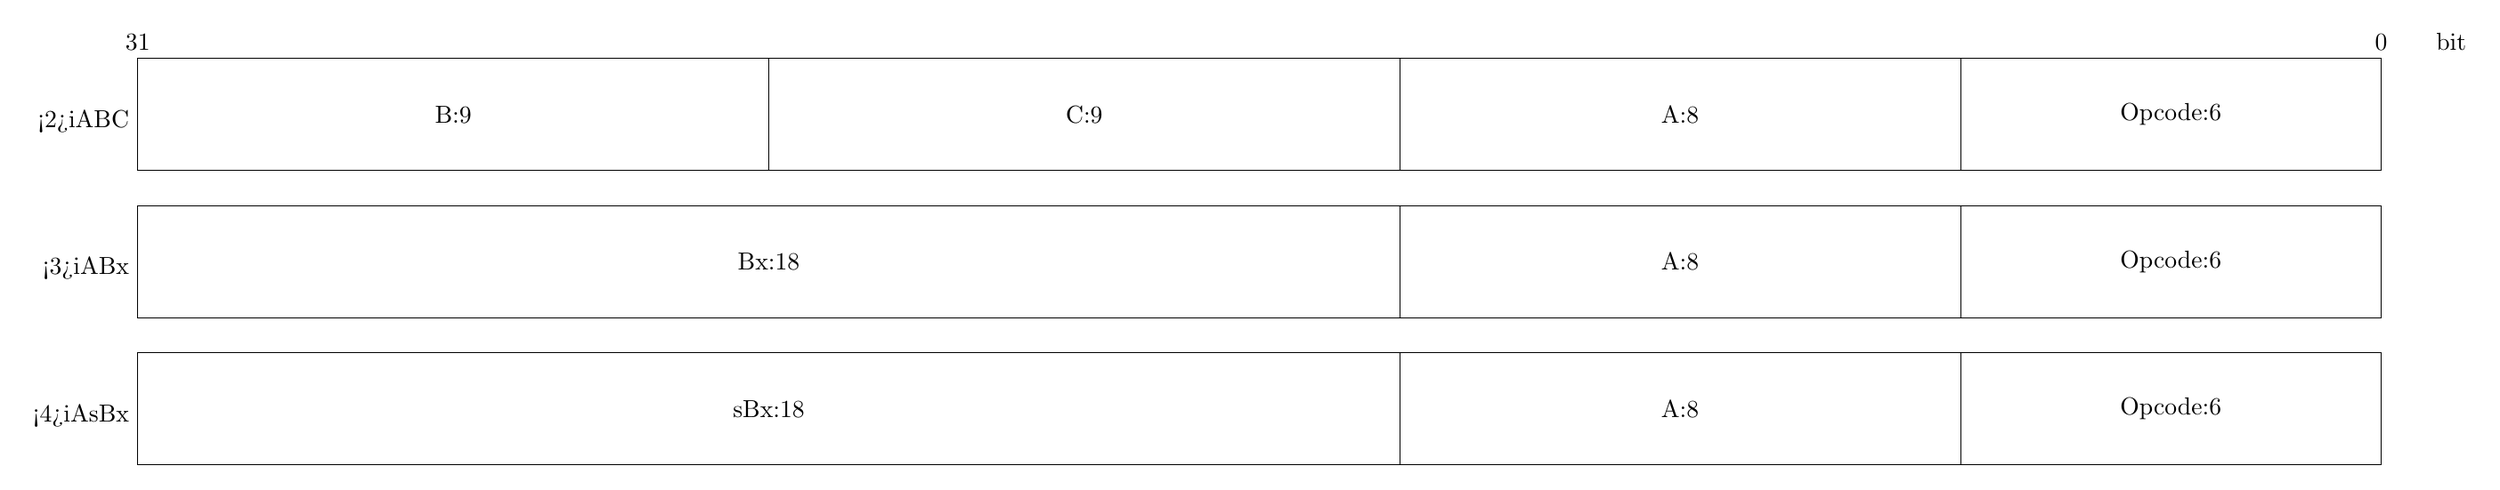
\begin{tikzpicture}
			\uncover<2->{\draw (0,0) node[above]{31};
				\draw (32\bitlen, 0) node[above]{0} (33\bitlen, 0) node[above]{bit};

				\draw (0, -.9\zw) node[left]{\alert<2>{iABC}};
				\draw (0,  -1.6\zw) rectangle (9\bitlen, 0) node[midway]{B:9};
				\draw (9\bitlen, -1.6\zw) rectangle (18\bitlen, 0) node[midway]{C:9};
				\draw (18\bitlen, -1.6\zw) rectangle (26\bitlen, 0) node[midway]{A:8};
				\draw (26\bitlen, -1.6\zw) rectangle (32\bitlen, 0) node[midway]{Opcode:6};}

			\uncover<3->{\draw (0,-3\zw) node[left]{\alert<3>{iABx}};
				\draw (0,  -3.7\zw) rectangle (18\bitlen, -2.1\zw) node[midway]{Bx:18};
				\draw (18\bitlen, -3.7\zw) rectangle (26\bitlen, -2.1\zw) node[midway]{A:8};
				\draw (26\bitlen, -3.7\zw) rectangle (32\bitlen, -2.1\zw) node[midway]{Opcode:6};}

			\uncover<4->{\draw (0,-5.1\zw) node[left]{\alert<4>{iAsBx}};
				\draw (0,  -5.8\zw) rectangle (18\bitlen, -4.2\zw) node[midway]{sBx:18};
				\draw (18\bitlen, -5.8\zw) rectangle (26\bitlen, -4.2\zw) node[midway]{A:8};
				\draw (26\bitlen, -5.8\zw) rectangle (32\bitlen, -4.2\zw) node[midway]{Opcode:6};}
		\end{tikzpicture}
	\end{table}
\end{frame}

\subsubsection{example}
\begin{frame}[fragile]{example}
	\begin{center}
		Q. \structure{この命令は?}

		\underline{1F 00 80 00 (\lstinline|funciton foo()|より)}
	\end{center}
	\begin{enumerate}
		\item<2-> endianを考慮しながらbitにする

			\uncover<3->{ヘッダの情報よりリトルエンディアン}
			\begin{center}
				\uncover<3->{%
					{1F 00 80 00 $\rightarrow$ 00 80 00 1F}%

					$\Downarrow$%
				}

				\uncover<4->{%
					\textcolor<5->{orange}{\ltjruby{0000000 1}{\uncover<7->{\small{}B}}}%
					\textcolor<5->{green}{\ltjruby{0000000 00}{\uncover<7->{\small{}C}}}%
					\textcolor<5->{orange}{\ltjruby{000000 00}{\uncover<7->{\small{}A}}}%
					\textcolor<5->{green}{\color<6->{blue}\ltjruby{011111}{\uncover<6->{\footnotesize{}RETURN}}}%
				}
			\end{center}
		\item<6-> Opcode 0b11111 は\textcolor{blue}{RETURN}
		\item<7-> \textcolor{blue}{RETURN}はiABC形式(ただしR(C)はnot used)
	\end{enumerate}
	\begin{center}
		\uncover<8->{A. \alert{RETURN 0 1 (0)}}
	\end{center}
\end{frame}
\begin{frame}[fragile]{example}
	\begin{center}
		Q. \structure{この命令をバイトコードに直すと? (little endian)}

		\underline{CALL 0 2 1}
	\end{center}
	\begin{enumerate}
		\item<2-> CALLはOpcode 0b11101
		\item<3-> iABC形式なので、32bitで以下のようになる

			\begin{center}
				\textcolor{orange}{\ltjruby{0000001 0}{{\small{}B}}}%
				\textcolor{green}{\ltjruby{0000000 01}{{\small{}C}}}%
				\textcolor{orange}{\ltjruby{000000 00}{{\small{}A}}}%
				\textcolor{blue}{\ltjruby{011101}{\footnotesize{}CALL}}%
			\end{center}
		\item<4-> little endianで16進数にしておわり
	\end{enumerate}
	\begin{center}
		\uncover<5->{A. \alert{1d 40 00 01}}
	\end{center}
\end{frame}
